% Introduction
% Author: Adnan Ghribi
\subsection{Background}

The \gls{spiral2} facility at \gls{ganil} in Caen, France (Fig.~\ref{fig:spiral2_overview}), represents a state-of-the-art particle accelerator designed for nuclear physics research and applications. The facility utilizes a superconducting \gls{linac} to deliver high-intensity, high-quality ion beams for experiments in nuclear structure, astrophysics, and fundamental interactions~\cite{orduz2024spiral2}.

\begin{figure}[h]
    \centering
    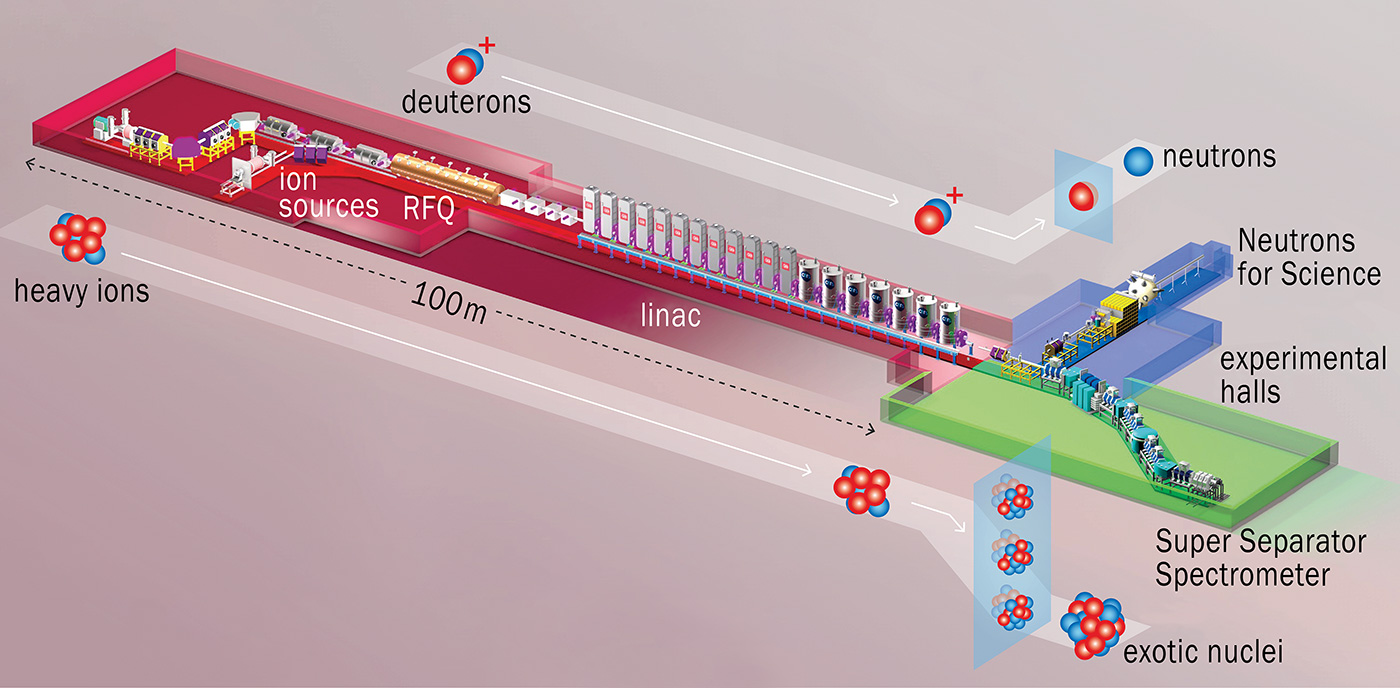
\includegraphics[width=\linewidth]{figures/spiral2.jpg}
    \caption{Overview of the SPIRAL2 accelerator facility at GANIL}
    \label{fig:spiral2_overview}
\end{figure}

A critical component of the \gls{spiral2} accelerator is the \gls{llrf} system \cite{bouly2022superconducting}, which regulates the electromagnetic fields in superconducting RF cavities to ensure precise beam acceleration and stability. The \gls{llrf} system continuously monitors 27 raw signals % MANUAL: real signal count, verified against features_engineered.pkl's signal_names list (Sec. 3), corrected from a wrong "16" here
including in-phase and quadrature (I/Q) components of cavity, reference, and incident RF signals, along with amplitudes, vacuum pressure, pickup currents, and control commands. From these raw measurements, key operational parameters are derived and controlled, including  cavity voltage amplitude ($U_{cav}$), cavity phase ($\Phi_{cav}$), forward power ($P_{fwd}$), reflected power ($P_{refl}$) and vacuum pressure ($P_{vac}$) (see Sec.~\ref{sec:system_description}). Maintaining these parameters within tight tolerances is essential for beam quality, operational efficiency, and equipment protection.

However, the \gls{llrf} system faces significant operational challenges. Complex fault scenarios can arise from hardware degradation, environmental fluctuations, beam loading effects, microphonics, and control loop instabilities. Multi-fault events, where multiple fault types occur simultaneously or in rapid succession, complicate diagnosis and recovery. Traditional threshold-based monitoring systems lack the sophistication to distinguish between fault types, identify root causes in multi-fault scenarios, or detect early warning signs (precursors) before faults fully develop.

\subsection{Motivation and Problem Statement}

Over the 2019--2025 % MANUAL: operational period per Classify_PostMortemFile/config.yaml's `years` list, not tied to a manifest metric
operational period, the \gls{spiral2} facility recorded \MetricZeroZeroDataAttritionChainVSixTotalEvents{} usable \gls{spiral2} postmortem events (after quality filtering; \MetricZeroZeroDataAttritionChainRawFiles{} raw postmortem files exist upstream) captured by the automated fault detection system and manual operator acquisitions. These events are classified into seven primary fault categories by a validated ground-truth classifier (\texttt{Classify\_PostMortemFile}, Sec.~\ref{sec:system_description}): \textbf{Pickup threshold} (\MetricZeroZeroDataAttritionChainGtPassingSeuilPickUp{} events), \textbf{Fast external cutoff} (\MetricZeroZeroDataAttritionChainGtPassingCoupureExterneRapide{} events), \textbf{RF authorization absent} (\MetricZeroZeroDataAttritionChainGtPassingAbsenceAutorisationRf{} events), \textbf{Vacuum threshold} (\MetricZeroZeroDataAttritionChainGtPassingSeuilDeVide{} events), \textbf{Cavity quench/breakdown} (\MetricZeroZeroDataAttritionChainGtPassingClaquageOuQuenchCavit{} events), \textbf{RF safety threshold exceeded} (\MetricZeroZeroDataAttritionChainGtPassingDPSeuilDeSCuritRf{} events), and \textbf{RF regulation out of tolerance} (\MetricZeroZeroDataAttritionChainGtPassingRGSignalRfHorsTolRance{} events). The dataset exhibits severe class imbalance -- a 54$\times$ ratio between the rarest and most common category % MANUAL: derived from the macro-cited event counts above (591/11 events), same ratio cited consistently in Sec. 3/6/7
-- addressed in this work through class-weighted training (Sec.~\ref{sec:methodology}) rather than assumed away.

The operational impact of these faults is substantial. Undiagnosed or misdiagnosed faults can lead to equipment damage and extended downtime for manual investigation and repair. Current manual fault diagnosis by expert operators is time-consuming, subject to human error, and reactive rather than proactive. There is a critical need for an automated, accurate, and interpretable fault diagnosis system that can:

\begin{enumerate}
    \item Detect anomalous events in real-time with high sensitivity
    \item Classify fault types in multi-label scenarios,
    \item Identify the root cause (primary fault) in multi-fault events,
    \item Detect fault precursors to enable preventive intervention,
    \item Provide explainable decisions for operator trust and system validation.
\end{enumerate}

Existing approaches in the literature (reviewed in Section~\ref{sec:related_work}) have addressed anomaly detection and fault classification in industrial systems, but few have tackled the specific challenges of root cause identification in multi-fault scenarios, precursor detection with quantifiable lead times, and physics-informed explainability in particle accelerator environments.

\subsection{Contributions}

This paper presents a comprehensive, integrated machine learning solution addressing these challenges, through the following key contributions:

\begin{enumerate}
    \item \textbf{Hybrid Multi-Phase Progressive Pipeline Architecture}: We design a modular pipeline that progressively increases in complexity, from unsupervised anomaly detection to supervised multi-label classification, root cause identification, and fault subtype clustering. This architecture enables targeted optimization at each stage while maintaining end-to-end coherence.

    \item \textbf{Physics-Informed Feature Engineering}: We develop \MetricZeroSixBinaryClassificationNFeatures{} features spanning statistical aggregations (mean, std, skewness, kurtosis), temporal characteristics (slopes, derivatives, CUSUM), and seven named physics-informed families (effective decay, detuning, microphonics, RF mismatch, modulator command, phase stability, RF power flow -- Appendix~\ref{appendix:features}), totaling \MetricOneZeroPhysicsGroupShapNFeaturesPhysicsInformedTotal{} of the \MetricZeroSixBinaryClassificationNFeatures{} features. % MANUAL: Statistical/Temporal counts are the real per-group feature-count macros cited in Sec. 4/5, simple arithmetic not a separate manifest metric here
A count-normalized SHAP analysis (Sec.~\ref{sec:explainability}) finds a physics-informed family dominant for four of seven fault categories -- a data-driven picture of which feature groups actually drive each fault category, and a materially different picture than the unnormalized group-sum comparison gives.

    \item \textbf{Root Cause Identification}: our Random Forest classifier achieves \MetricZeroEightPhaseThreeaRootcauseStabilityAccuracyMean\ $\pm$ \MetricZeroEightPhaseThreeaRootcauseStabilityAccuracyStd\ accuracy (repeated-split mean $\pm$ std, 10 splits % MANUAL: n_repeats=10 is a fixed constant in every repeated_leakage_safe_eval() call this session, not itself a manifest metric
) identifying the primary fault among \MetricZeroEightPhaseThreeaRootcauseNFaultEvents{} fault events, addressing a gap in existing literature. Per-category F1 ranges from \MetricZeroEightPhaseThreeaRootcauseStabilityPerLabelFOneCoupureExterneRapideMean\ for the rarest category (\MetricZeroZeroDataAttritionChainGtPassingCoupureExterneRapide{} events) to \MetricZeroEightPhaseThreeaRootcauseStabilityPerLabelFOneDPSeuilDeSCuritRFMean\ for well-populated categories -- this spread, not a single averaged number, is what class imbalance actually costs.

    \item \textbf{Fault Subtype Discovery}: unsupervised clustering within each fault category (Step 09) % MANUAL: "Step 09" names the pipeline step, not a result metric
finds a consistent best $k=\MetricZeroNinecEnhancedSubclassDiscoveryRfAuthorizationAbsentBestK$ substructure in every one of the \MetricZeroNinecEnhancedSubclassDiscoveryNCategoriesAnalyzed{} categories with enough events to cluster reliably (silhouette \MetricZeroNinecEnhancedSubclassDiscoveryCavityQuenchBreakdownSilhouette--\MetricZeroNinecEnhancedSubclassDiscoveryVacuumThresholdSilhouette); the remaining \MetricZeroZeroDataAttritionChainGtPassingSeuilPickUp- and \MetricZeroZeroDataAttritionChainGtPassingCoupureExterneRapide-event categories lack sufficient data for this analysis. These subtypes reveal bimodal operational patterns not captured by top-level fault labels.

    \item \textbf{Early Fault-Onset Detection Ahead of the Interlock Trip}: our corrected precursor model (trained only on features from a fixed window before each event's own trigger, guarding against post-trigger leakage) reaches \MetricZeroFivePhaseZeroPrecursorRandomForestRocAuc\ ROC AUC, remaining confident at least \MetricZeroFivePrecursorLeadTimeLeadTimeMsLowerBoundMeanCensored{}ms before the interlock trip for every sampled true-positive event -- a lower bound, not a fully characterized lead time; we report this measurement as right-censored rather than asserting a specific window.

    \item \textbf{Explainability Framework}: we integrate SHAP (global and local feature importance) and LIME (instance-level explanations) to provide multi-level interpretability, validated against known LLRF physics.

    \item \textbf{Offline Exploratory Analysis with a Real Latency Benchmark}: the modular pipeline architecture demonstrates the feasibility of automated fault diagnosis on postmortem LLRF data. Measured single-event inference time (mean, single-threaded, no batching) is \MetricInferenceLatencyBenchmarkStepZeroSixBinaryRfMeanMs{}ms for binary classification and \MetricInferenceLatencyBenchmarkPhaseCLabelPowersetMeanMs{}ms for the best multi-label approach, suggesting feasibility for future real-time integration with monitoring infrastructure.
\end{enumerate}

\subsection{Paper Organization}

The remainder of this paper is organized as follows. Section~\ref{sec:related_work} reviews related work in anomaly detection and fault diagnosis for \gls{llrf} in particle accelerators. Section~\ref{sec:system_description} describes the \gls{spiral2} \gls{llrf} system, dataset characteristics, and data acquisition procedures. Section~\ref{sec:methodology} presents the pipeline architecture in detail, covering each step from data loading through the results-manifest sync mechanism that keeps this report's numbers traceable to the code. Section~\ref{sec:explainability} discusses the explainability and interpretability framework. Section~\ref{sec:results} reports headline performance across every re-verified step, the physics-group SHAP breakdown, and a real inference-latency benchmark. Section~\ref{sec:discussion} discusses key findings, practical implications, and limitations. Section~\ref{sec:conclusion} concludes with a summary of contributions and future research directions. Appendices provide complete feature definitions, hyperparameter settings, and additional experimental results.